\documentclass[11pt]{article}
\usepackage[a4paper, margin=2.5cm]{geometry}
\usepackage{amsmath, amssymb, amsthm}
\usepackage{graphicx}
\usepackage{booktabs}
\usepackage{multirow}
\usepackage{hyperref}
\usepackage{tikz}
\usetikzlibrary{arrows.meta, positioning}

\title{An Example Academic Article Template}
\author{First Author \and Second Author}
\date{\today}

\begin{document}
\maketitle

\begin{abstract}
This template demonstrates a typical academic article layout: sections,
mathematical equations, figures drawn with TikZ, professional tables with
\texttt{booktabs}, and a bibliography. Replace the content with your own work.
\end{abstract}

\section{Introduction}
Academic writing benefits from a clean separation between content and
presentation. \LaTeX{} excels at typesetting mathematics such as
\begin{equation}
  \nabla \cdot \mathbf{E} = \frac{\rho}{\varepsilon_0},
  \qquad
  \nabla \times \mathbf{B} = \mu_0 \mathbf{J} + \mu_0 \varepsilon_0
  \frac{\partial \mathbf{E}}{\partial t}.
\end{equation}
Inline math like $\alpha$, $\beta$, and $\sum_{i=1}^{n} x_i$ flows naturally
within the text.

\section{Method}
Figure~\ref{fig:pipeline} shows a simple pipeline rendered with TikZ, so the
template compiles out of the box without external image files.

\begin{figure}[htbp]
  \centering
  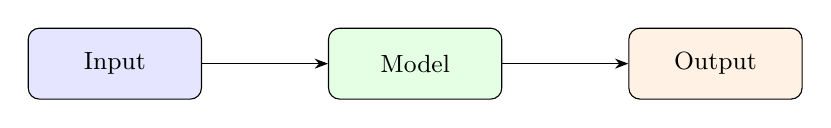
\begin{tikzpicture}[node distance=1.6cm, every node/.style={font=\small}]
    \node[draw, rounded corners, fill=blue!10, minimum width=2.2cm, minimum height=0.9cm] (input) {Input};
    \node[draw, rounded corners, fill=green!10, minimum width=2.2cm, minimum height=0.9cm, right=of input] (model) {Model};
    \node[draw, rounded corners, fill=orange!10, minimum width=2.2cm, minimum height=0.9cm, right=of model] (output) {Output};
    \draw[-{Stealth}] (input) -- (model);
    \draw[-{Stealth}] (model) -- (output);
  \end{tikzpicture}
  \caption{A TikZ-drawn pipeline: no external images required.}
  \label{fig:pipeline}
\end{figure}

\section{Experiments}
Table~\ref{tab:results} reports illustrative results using \texttt{booktabs}
rules for a professional look.

\begin{table}[htbp]
  \centering
  \caption{Example results table.}
  \label{tab:results}
  \begin{tabular}{lccc}
    \toprule
    Method & Accuracy (\%) & F1 & Latency (ms) \\
    \midrule
    Baseline        & 81.2 & 0.79 & 12 \\
    + Augmentation  & 84.6 & 0.83 & 13 \\
    Ours            & \textbf{88.1} & \textbf{0.87} & 15 \\
    \bottomrule
  \end{tabular}
\end{table}

\section{Conclusion}
This template provides a solid starting point. Cite works like~\cite{knuth1984}
and~\cite{lamport1994} using \verb|\cite{}|.

\begin{thebibliography}{9}
\bibitem{knuth1984}
Donald E. Knuth.
\newblock \emph{The TeXbook}.
\newblock Addison-Wesley, 1984.

\bibitem{lamport1994}
Leslie Lamport.
\newblock \emph{\LaTeX: A Document Preparation System}.
\newblock 2nd edition, Addison-Wesley, 1994.
\end{thebibliography}

\end{document}
